\chapter{PROSES DAN PENGEMBANGAN DESAIN}

% Bab Studi Literatur digunakan untuk mendeskripsikan kajian literatur yang terkait dengan persoalan tugas akhir. Tujuan studi literatur adalah:

% \begin{enumerate}
%     \item menunjukkan kepada pembaca adanya gap seperti pada rumusan masalah yang memang belum terselesaikan,
%     \item memberikan pemahaman yang secukupnya kepada pembaca tentang teori atau pekerjaan terkait yang terkait langsung dengan penyelesaian persoalan, serta
%     \item menyampaikan informasi apa saja yang sudah ditulis/dilaporkan oleh pihak lain (peneliti/Tugas Akhir/Tesis) tentang hasil penelitian/pekerjaan mereka yang sama atau mirip kaitannya dengan persoalan tugas akhir.
% \end{enumerate}

\section{Tinjauan Pustaka}
% Resource Allocator (VideoStorm)
% VAP (DDS)
% Tools (gRPC, tc, python, linux)

    \subsection{Resource Allocator}
    Kehadiran sebuah \textit{resource allocator} merupakan hal yang sangat krusial pada keberlangsungan sistem \textit{edge computing}. Keterbatasan sumber daya komputasi merupakan motivasi
    utama dibalik kebutuhan sistem ini. Sumber daya komputasi harus secara cerdas dan tepat dialokasikan sesuai dengan kebutuhan perangkat \textit{edge} 
    sehingga tidak terdapat \textit{backlog} yang dapat menurukan performansi \citep{edgeComp2}.
    Sumber daya komputasi yang bisa dialokasikan berupa \gls{cpu}, \gls{gpu}, \textit{bandwidth}, \textit{memory}, dan \textit{storage} \citep{edgeCompDis}.

    Beberapa peneliti sudah mengajukan sistem \textit{resource allocator}, diantaranya adalah VideoStorm \citep{videostorm}, \gls{jcab} \citep{jcab}, dan AutoML \textit{for \gls{vap}} \citep{automl}.
    \gls{jcab} melakukan alokasi berdasarkan \textit{bandwidth} dan model \gls{cnn}, artinya pada suatu sistem, terdapat beberapa model yang di-\textit{deploy} berdasarkan resolusi video masukan. 
    Tiap kumpulan video akan didistribusikan pada model \gls{cnn} yang berbeda-beda mengikuti konfigurasi video yang sudah ditentukan sebelumnya.

    Sementara AutoML \textit{for \gls{vap}} adalah sebuah \textit{framework} AutoML yang sengaja dibuat untuk memilih konfigurasi yang teroptimasi untuk \gls{vap} dan pembuatan model \gls{cnn}. VideoStorm, di lain sisi
    adalah sebuah \textit{resource allocator} yang melakukan alokasi terhadap \textit{bandwidth}. Cara kerja VideoStorm adalah pertama-tama kamera-kamera akan mengirimkan video kepada server.
    Lalu pada suatu periode tertentu, VideoStorm akan melakukan alokasi \textit{bandwidth} dengan menganalisis hasil dari beberapa detik sebelumnya dan menentukan \textit{bandwidth} yang sesuai dengan kebutuhannya.
    
    \subsection{Video Analytics Application}

    Faktor utama keberhasilan sebuah sistem \textit{Video Analytics} selaras dengan \textit{Video Analytics Application} (\gls{vap}) yang digunakan. Semakin cerdas \gls{vap}
    maka akan semakin baik performansi yang dihasilkan oleh sistem. \citep{killer} mengatakan bahwa \gls{vap} merupakan sistem yang sangat kompleks jika ingin diterapkan pada jaringan \textit{edge}.
    Hal ini diakibatkan oleh video yang memiliki ukuran data yang relatif besar dan waktu pemrosesan yang cukup lama. Sehingga diperlukan pertimbangan yang sangat matang dalam mendesain sebuah \gls{vap}.

    Sebuah sistem \gls{vap} terdiri dari \textit{client}, \textit{middleware}, dan \textit{server}. \textit{Client} biasanya berupa kamera yang digunakan untuk menangkap video dan melakukan beberapa proses seperti \textit{encoding}
    untuk dikirimkan kepada \textit{server}. \textit{Middleware} adalah sebuah sistem yang menghubungkan \textit{client} dengan \textit{server} yang berfungsi untuk menjamin keberlangsungan transmisi data antar keduanya \citep{middleware}.
    Sementara \textit{server} berguna untuk memproses data seperti melakukan deteksi objek, mengklasifikasikan objek, atau melakukan kegiatan komputasi lainnya.

    Beberapa \gls{vap} sudah diajukan diantaranya adalah \gls{dds} \citep{dds}, AWStream \citep{aws}, Reducto \citep{reducto}, dan Glimpse \citep{glimpse}.
    \gls{dds} adalah sebuah \gls{vap} yang bekerja dengan cara mengirim video menggunakan 2 kali iterasi sehingga dapat diperoleh hasil yang baik. Salah satu persyaratan dalam mendesain \gls{vap}
    adalah \textit{self-adaptability} \citep{chameleon}, hal ini bermakna bahwa \gls{vap} dapat beradaptasi dengan kondisi lingkungannya dengan cara mengubah konfigurasi videonya.

    % Float adalah \textit{container} untuk elemen-elemen dokumen yang tidak dapat dipisah menjadi beberapa halaman. Environment ``table'' dan ``figure'' secara default adalah float. Float berguna untuk memudahkan peletakan objek yang tidak cukup jika diletakkan di halaman sekarang. Peletakan float diatur oleh \LaTeX\ dan pengguna sebaiknya memberikan keleluasaan kepada \LaTeX\ agar dapat mengatur peletakan dengan baik. 
    
    \subsection{Traffic Control}
    \textit{Traffic control} atau lebih dikenal dengan tc adalah sebuah \textit{tools} pada linux yang dapat digunakan untuk memegang kendali atas trafik pada kernel linux \citep{tc}.
    Beberapa fungsi utama dari tc adalah \textit{SHAPING}, \textit{SCHEDULING}, \textit{POLICING}, dan \textit{DROPPING}.

    Salah satu \textit{use-case} yang paling sering digunakan yakni tc akan digunakan sebagai alat yang dapat mengontrol transmisi dari sebuah \textit{interface} jaringan,
    salah satunya adalah untuk menurunkan atau mengelompokan  \textit{ingress bandwidth} ke beberapa \textit{virtual interface} sehingga kelakuannya dapat dikontrol.

    \subsection{gRPC}
    gRPC adalah sebuah \textit{framework} RPC atau \textit{Remote Procedure Call} \textit{open source} universal yang dikembangkan oleh Google \citep{grpc}.
    gRPC digunakan sebagai \textit{tools} penghubung antar perangkat atau perangkat dengan \textit{server} yang dapat dicopot pasang secara mudah.
    % \includesvg{./resources/grpc.svg}
    \begin{figure}[tbh]
        \centering
        \includesvg[scale=0.75]{./resources/grpc.svg}
        \caption{Use-Case gRPC \citep{grpc}}\label{fig:gRPC}
    \end{figure}

    gRPC adalah \textit{framework} RPC yang universal, hal ini bermakna bahwa gRPC mendukung komunikasi data menggunakan bahasa pemrograman yang berbeda
    seperti yang ditunjukan pada Gambar \ref{fig:gRPC}. gRPC menggunakan \textit{Protocol Buffers} atau protobuf sebagai struktur data pada pesan yang dikirimkan,
    secara sekilas, protobuf mirip seperti JSON, namun protobuf universal, lebih ringan, dan lebih cepat dari segi performansi.

    gRPC mendukung berbagai macam jenis komunikasi yakni
    \begin{enumerate}
        \item \textit{Unary RPC} yaitu \textit{client} akan mengirimkan sebuah \textit{request} dan \textit{server} akan mengirimkan sebuah respon. Pada komunikasi ini, hanya \textit{server} yang dapat mengirimkan respon, tidak berlaku sebaliknya
        \item \textit{Server streaming RPC} yaitu \textit{client} akan mengirimkan sebuah \textit{request} dan \textit{server} akan mengirimkan respon yang tak henti hingga pesannya selesai.
        \item \textit{Client streaming RPC} yaitu kebalikannya dari \textit{Server streaming RPC}, yakni \textit{server} yang akan melakukan \textit{request} dan \textit{client} yang akan mengirimkan pesan tak henti.
        \item \textit{Bidirectional streaming RPC} yaitu \textit{client} dan \textit{server} dapat mengirim \textit{request} dan mendapat respon dari satu sama lain
    \end{enumerate}
    % \subsection{Python}
    % \subsection{Linux}
    % \subsubsection{Gambar}
    
    % Float bisa di-\textit{cross reference}. Contohnya Gambar~\ref{fig:contoh_gambar} adalah contoh gambar.

    % \begin{figure}[h]
    %     \centering
    %     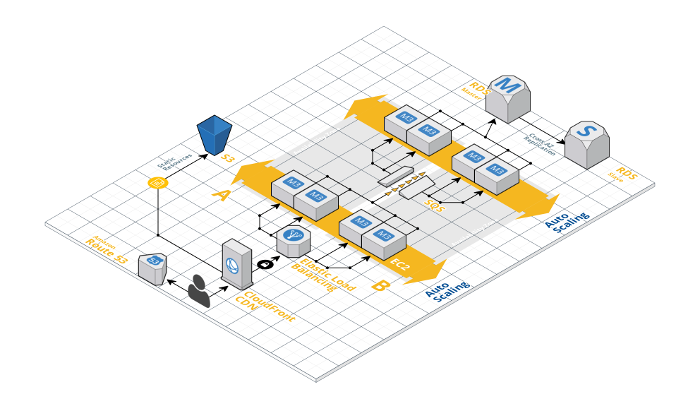
\includegraphics[width=0.8\textwidth]{resources/chapter-2-infrastructure-diagram.png}
    %     \caption{Contoh gambar}
    %     \label{fig:contoh_gambar}
    % \end{figure}

    % \subsubsection{Tabel}

    % Tabel juga merupakan float. Tabel~\ref{table:contoh_tabel} adalah contoh tabel.

    % \begin{table}[htbp]
    %     \small
    %     \centering
    %     \caption{Contoh Tabel}
    %     \label{table:contoh_tabel}
    %     \begin{tabular}{ll}
    %         \toprule
    %         \multicolumn{1}{l}{\textbf{Contoh Judul Kolom}} & \multicolumn{1}{l}{\textbf{Nilai}}\\
    %         \midrule
    %         Besaran 1 & 12 meter          \\
    %         Besaran 2 & $360^\circ$       \\
    %         Besaran 3 & 0,2 meter         \\
    %         Besaran 4 & $1^\circ$         \\
    %         Besaran 5 & 8000 sampel/detik \\
    %         \bottomrule
    %     \end{tabular}
    % \end{table}

    % \subsection{Persamaan Matematika}

    % \blindtext Persamaan~\eqref{eq:contoh_equation} adalah contoh persamaan matematika,

    % \begin{align}
    %     c^2 = a^2 + b^2\,.
    % \label{eq:contoh_equation}
    % \end{align}
    
    % Contoh penggunaan notasi custom,
    
    % \begin{align}
    %     \bayes{x}{y}\,.
    % \label{eq:contoh_equation_custom}
    % \end{align}

\section{Persyaratan Desain}
    \textit{Resource allocator} yang dirancang akan diintegrasikan dengan sebuah \gls{vap} terbaik dari segi performansi yakni \gls{dds}.
    Berdasarkan II.x, harus bisa memenuhi rancangan sebagai berikut. Ini nanti dielaborasiin lagi. Diturunin objektif seperti berikut
    \begin{enumerate}
        \item \textit{Resource allocator} bersifat real-time (\textit{Real-time design})
        \item \textit{Resource allocator} harus bisa melakukan tradeoff yang minimal antara bandwidth dan akurasi (\textit{Optimal Trade-off})
        \item \textit{Resource allocator} memiliki harga pengembangan yang minimal (\textit{Minimum Costs})
    \end{enumerate}

    Dari objektif tersebut, diturunkan subobjektif sebagai berikut. Bla Bla
    % Comment this block if not needed
    \begin{figure}[tbh]
        \centering
        \includesvg[scale=0.8]{./resources/Obj_Tree.svg}
        \caption{Objective Tree}\label{fig:obj_tree}
    \end{figure}

    \begin{center}
        \begin{tabular}{|m{9cm}|}
            \hline

            % (\begin{itemize}
            %     \item Objektif 1: \textit{Real-time Design}
            % \end{itemize})\\
            % Lorem Ipsum \\
            \begin{outline}
                \1[$\bullet$] Objektif 1: \textit{Real-time Design}
                    \2[$\circ$] Subojektif 1: Latensi Minimum
                \1[$\bullet$] Objektif 2: \textit{Trade-off} optimal 
                    \2[$\circ$] Subobjektif 2: Alokasi \textit{bandwidth} terhadap akurasi \textit{inference}
                \1[$\bullet$] Objektif 3: Harga minimum 
                    \2[$\circ$] Subobjektif 3: Sistem operasi yang bersifat \textit{open source}
            \end{outline}\\
            \hline
        \end{tabular}
    \end{center}

    Dari subobjektif tersebut, lahirlah constraint sebagai berikut

    \begin{center}
        \begin{tabular}{|m{12cm}|}
            \hline
            \begin{outline}
                \1[$\bullet$] Objektif 1: \textit{Real-time Design}
                    \2[$\circ$] Subojektif 1: Latensi Minimum
                        \3[$\centerdot$] \textit{Constraint}: Latensi E2E tidak melebihi 1 detik
                \1[$\bullet$] Objektif 2: \textit{Trade-off} optimal 
                    \2[$\circ$] Subobjektif 2: Alokasi \textit{bandwidth} terhadap akurasi \textit{inference}
                        \3[$\centerdot$] \textit{Constraint}: Ketersediaan \textit{bandwidth} yang terbatas untuk klien sumber video
                \1[$\bullet$] Objektif 3: Harga minimum 
                    \2[$\circ$] Subobjektif 3: Sistem operasi yang bersifat \textit{open source}
                        \3[$\centerdot$] \textit{Constraint}: Harus menggunakan sistem operasi Linux
            \end{outline}\\
            \hline
        \end{tabular}
    \end{center}

    trs lahir ini deh Fungsional

    \begin{center}
        \begin{tabular}{|m{5cm}|m{4cm}|m{3cm}|}
            \hline
            \thead{Subobjektif dan \textit{Constraint}} &  \thead{Persyaratan Fungsional} & \thead{Fungsi} \\
            \hline
            \begin{outline}
                \0 \textbf{Subobjektif 1}: Latensi Minimum
                    \1[] \textbf{\textit{Constraint}}: Latensi E2E tidak melebihi 1 detik
                \0 \textbf{Subobjektif 2}: Alokasi \textit{bandwidth} terhadap akurasi \textit{inference}
                    \1[] \textbf{\textit{Constraint}}: Ketersediaan \textit{bandwidth} yang terbatas untuk klien sumber video
                \0 \textbf{Subobjektif 3}: Sistem operasi yang bersifat \textit{open source}
                    \1[] \textbf{\textit{Constraint}}: Harus menggunakan sistem operasi Linux
            \end{outline} & 
            \begin{enumerate}
                \item Latensi E2E (end-to-end)
                pada sistem tidak lebih
                dari 1 detik untuk
                menghindari terjadinya
                backlog saat pengukuran overhead
                \item Kebutuhan alokasi efisien
                terhadap ketersediaan
                bandwidth yang terbatas
                untuk mencapai nilai
                akurasi inferensi yang
                terbaik
                \item Linux digunakan sebagai
                operating system karena
                beberapa program hanya
                dapat berjalan pada OS
                tersebut (contohnya: TC)
            \end{enumerate} & \begin{enumerate}
                \item lorem
            \end{enumerate} \\
            \hline
        \end{tabular}
    \end{center}

\section{Konsep Desain}
\section{Pengembangan Desain}
\blindtext
